%%% Local Variables: 
%%% mode: latex
%%% TeX-master: "../../master"
%%% End: 
%%% introduction.tex --- 

%% Author: garamonfok@gros
%% Version: $Id: introduction.tex,v 0.0 2011/10/09 18:39:32 garamonfok Exp$

\section{Introduction}

The analysis of adaptation at large or complete genome scale is currently based on concepts and methods developed for single genes analyzes \cite{Arbiza2006,Bakewell2007,Bustamante2005,Clark2003,Nielsen2005}. Statistical methods to test for neutrality \cite{Nielsen2001}, are currently used without considering if genes works independently or associated to others to produce a single phenotypic response. In this sense we are applying pre-genomics concepts and methods to genomics data. The current paradigm for large scale analysis of adaptation consists in a two steps framework: first, the search for a list of genes (in a gene-by-gene framework analysis) with a statistical significant signal of positive selection ($\omega > 1$), and second, the search for over-represented functional classes of genes in this list. Although it is logically consistent, it has been noted that this kind of strategy causes an enormous loss of information due to the large number of false negatives that are accepted in order to preserve a low ratio of false positives necessary when genomics data is considered \cite{Al-Shahrour2007,Al-Shahrour2005a,Al-Shahrour2006,Subramanian2005}.

Genes do not operate alone within the cell, but in a intricate network of interactions that we have only recently started to envisage \cite{Stelzl2005}. It is a widely accepted fact that coexpressing genes tend to be fulfilling common roles in the cell \cite{Lee2003}. Moreover, coexpression seems to occur, in many cases, in contiguous chromosomal regions \cite{Caron2001} and furthermore, recent evidences suggest that functionally related genes map close in the genome, even in higher eukaryotes \cite{Hurst2004}. Many higher-order levels of interaction are continuously being discovered and even complex traits, including diseases, have started to be considered from a systems biology perspective \cite{Ideker2008}.

Recent studies stress the correlated change of positively selected genes working together through biochemical pathways (Caroline de Cornell) or through the protein-protein network interactions (citar reciente BMC de Yang). Moreover, a recent methodology was proposed to circumvent the classical two-step analysis as a new attempt to test for selective signatures across species at genome-scale level \cite{Shapiro2008} Using the deviations of the expected rates of evolution for a large group of genes in a group of gamma proteobacteria, the authors conclude that the coherence of selective patterns suggests that the genomic landscape is organized into functional modules even at the level of natural selection. Similar conclusions have been reported by Kosakovsky Pond, et al (citar PNAS secreto) which demonstrated that genes within the same functional group tend to exhibit similar evolutionary patterns within and between viral genomes.

The hypothesis we aim to test in this study is not about individual genes, but about functional classes. Mutations occur on single genes but natural selection acts on phenotypes by operating on whole sub-cellular systems. Mutations in genes either remain finally fixed or disappear because of their beneficial or disadvantageous effect on individual fitness, respectively. This effect on the function of individual proteins can only be understood in the context of the system (e.g. a pathway, GO functional roles, etc.) in which the proteins are involved. If a list of genes arranged by some parameter that accounts for their evolutionary rates is examined, it is expected that genes belonging to pathways or functional classes favored or disfavored by selection will tend to appear towards the extremes.

This approach circumvents the implicit assumption posed by the two-step analysis described above assuming by that the gene is the only target of selection. If natural selection works by means of minor quantitative effects of many different changes distributed along different gene products most of them working together in a few number of systems (GO functional terms, biochemical pathways and/or interactome modules) we expect to find: \begin{inparaenum}[ 1-] \item correlated nonsynonymous rate changes associated to these functions , \item synonymous rate changes not necessarily associated to the same functions, \item a higher number of significant functions than those discovered in the classical two-step approach.\end{inparaenum}

In the first part of this paper we extend the classical two-step approach previously reported by us for human and chimp \cite{Arbiza2006}, to rat and mouse now considering a set of XXXX orthologous genes of human, chimpanzee, mouse, rat and dog. The objective is to compare the classical two-step approach with the new system approach developed in the second part of the paper. In both cases we search for differences in evolutionary rates differentiating positive selection from relaxation along the branches of the phylogeny of the species.

\section{Material and Methods}

\subsection{Dataset}

\subsubsection{Five mammals}

Complete genomes of 5 mammals species (\textit{Homo sapiens}, \textit{Pan troglodytes}, \textit{Mus musculus}, \textit{Rattus norvegicus} and \textit{Canis familiaris}) where retrieved from \textit{Ensembl} \cite{Flicek2011}. Also orthology prediction between each pair of species
possibly done between human and the others was retrieved from \textit{Ensembl Compara} \cite{Vilella2009} using biomart \cite{Kinsella2011}. Only groups of orthologs \textit{one-to-one} with one representative of each species where kept in the final dataset. \fref{fig:phylogeny}{}
NUMBERS

\subsubsection{6 Drosophila}

\subsection{Alignments}
Each of the group of orthologous sequences were aligned with Muscle \cite{Edgar2004}, and, once aligned sequences were cleaned with trimal \cite{Capella-Gutierrez2009} keeping all sequences but trimming aligment columns with the euristic1 method.


\begin{figure}[htpb] 
\centering 
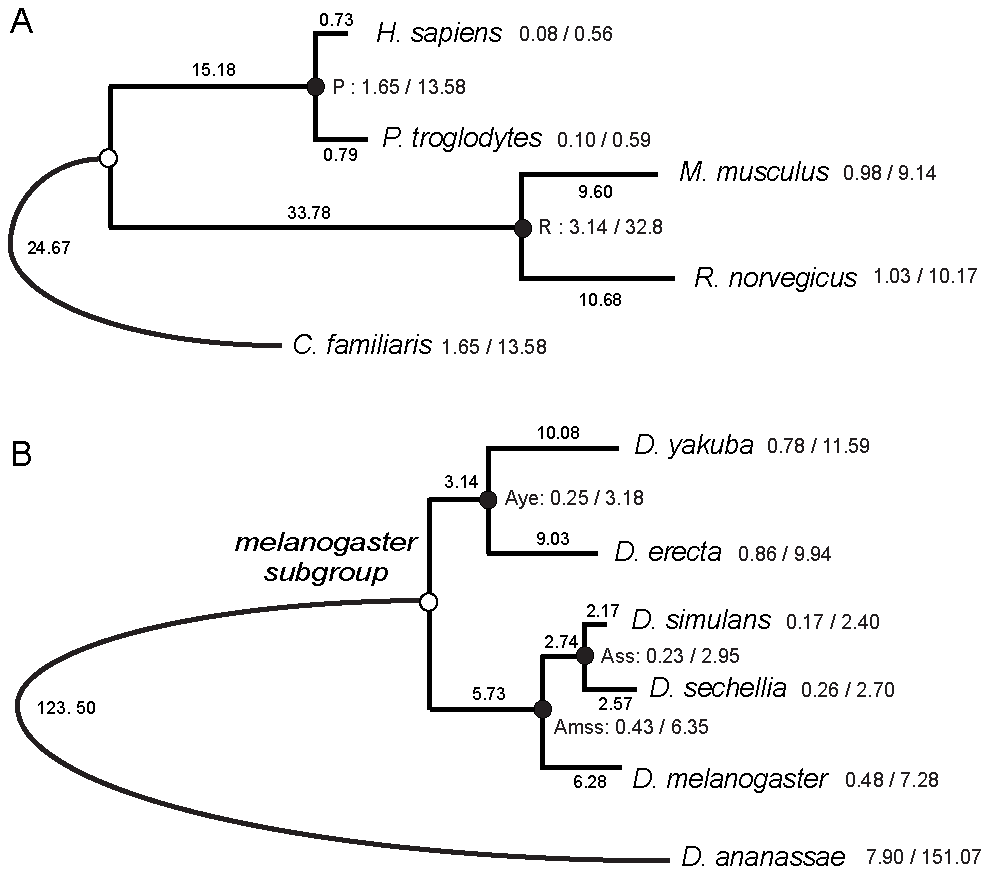
\includegraphics[width=\textwidth]{tex_source/figures/gssa/phylogenies.png}
\caption[Mammals and \textit{Drosophila} phylogeny]{{\bf Mammals and
  \textit{Drosophila} phylogeny.} \\blabli blob lu dkfnlskjdf blabli blob lu dkfnlskjdf blabli blob lu dkfnlskjdf blabli blob lu dkfnlskjdf blabli blob lu dkfnlskjdf blabli blob lu dkfnlskjdf  blob lu dkfnlskjdf blabli blob lu dkfnlskjdf blabli blob lu dkfnlskjdf} 
\label{fig:phylogeny}
\end{figure}


\section{open on colocalization to not random}

